\notechapter{N-20251217}{A Nontrivial Loop at Zero: FinSet K-Theory and Stable Homotopy}

\section{Why this second note exists}

This note is the corrected version of the earlier summer memo.  The first reaction to the line
\[
  0=1-1=-1+1=0
\]
was to think about analytic regularization: Ces\`aro summation, Abel summation, or the familiar divergent series
\[
  1-1+1-1+\cdots.
\]
Another tempting guess was the Eilenberg swindle: maybe an infinite object absorbs a copy of itself, so that something becomes zero by shifting parentheses at infinity.

After finding the actual lecture slides, the point became clearer.  The lecture is not about assigning a numerical value to a divergent expression.  It is about a process.  The equality \(0=0\) is not the content.  The content is the particular way in which \(0\) travels to \(0\).  In higher-categorical language, equality is no longer only a proposition; it carries paths, loops, and higher structure.

So the slogan of this note is:
\[
  \text{the important object is not the endpoint \(0\), but the loop based at \(0\).}
\]
The loop is created by making a \(+\) and a \(-\), swapping them, and annihilating them again:
\[
  \varnothing
  \sim
  \{+,-\}
  \sim
  \{-,+\}
  \sim
  \varnothing.
\]
Under the \(K\)-theory of finite sets, this loop becomes a nontrivial element.  Under the Barratt--Priddy--Quillen theorem, it corresponds to the stable Hopf class.

\section{The lecture starts from ordinary equations}

The slide deck begins with familiar equations: Pythagoras, Euler's identity, Stokes' theorem, the Navier--Stokes equation, the Langlands slogan, and then the strange meme equation.  This is pedagogically important.  It suggests that an equation is not merely a string of symbols with a truth value.  An equation may also encode a method, a structure, or a path.

In elementary arithmetic,
\[
  0=1-1=-1+1=0
\]
is boring.  Both sides are zero.  But the lecture asks us to stop looking only at the value.  In a higher structure, there can be more than one way for an object to equal itself.  The identity loop at \(0\) and the creation--swap--annihilation loop at \(0\) need not be the same.

\begin{remark}
This is the conceptual bridge to homotopy type theory and higher category theory.  A statement \(a=b\) can be represented by a path from \(a\) to \(b\).  Then two proofs of equality may themselves be compared by a homotopy.  The lecture uses this philosophy in a concrete topological model rather than as formal type theory.
\end{remark}

\section{The Hopf fibration as the first nontrivial map}

The first mathematical anchor is the Hopf fibration.  Define
\[
  S^3=\{(z_1,z_2)\in\mathbb C^2: |z_1|^2+|z_2|^2=1\}.
\]
The Hopf map is
\[
  H:S^3\to \mathbb{CP}^1\cong S^2,
  \qquad
  (z_1,z_2)\mapsto [z_1:z_2].
\]
For every point of \(S^2\), its preimage is a circle.  These circles are linked in a highly organized way.

\Needspace{16\baselineskip}
\begin{figure}[htbp]
  \centering
  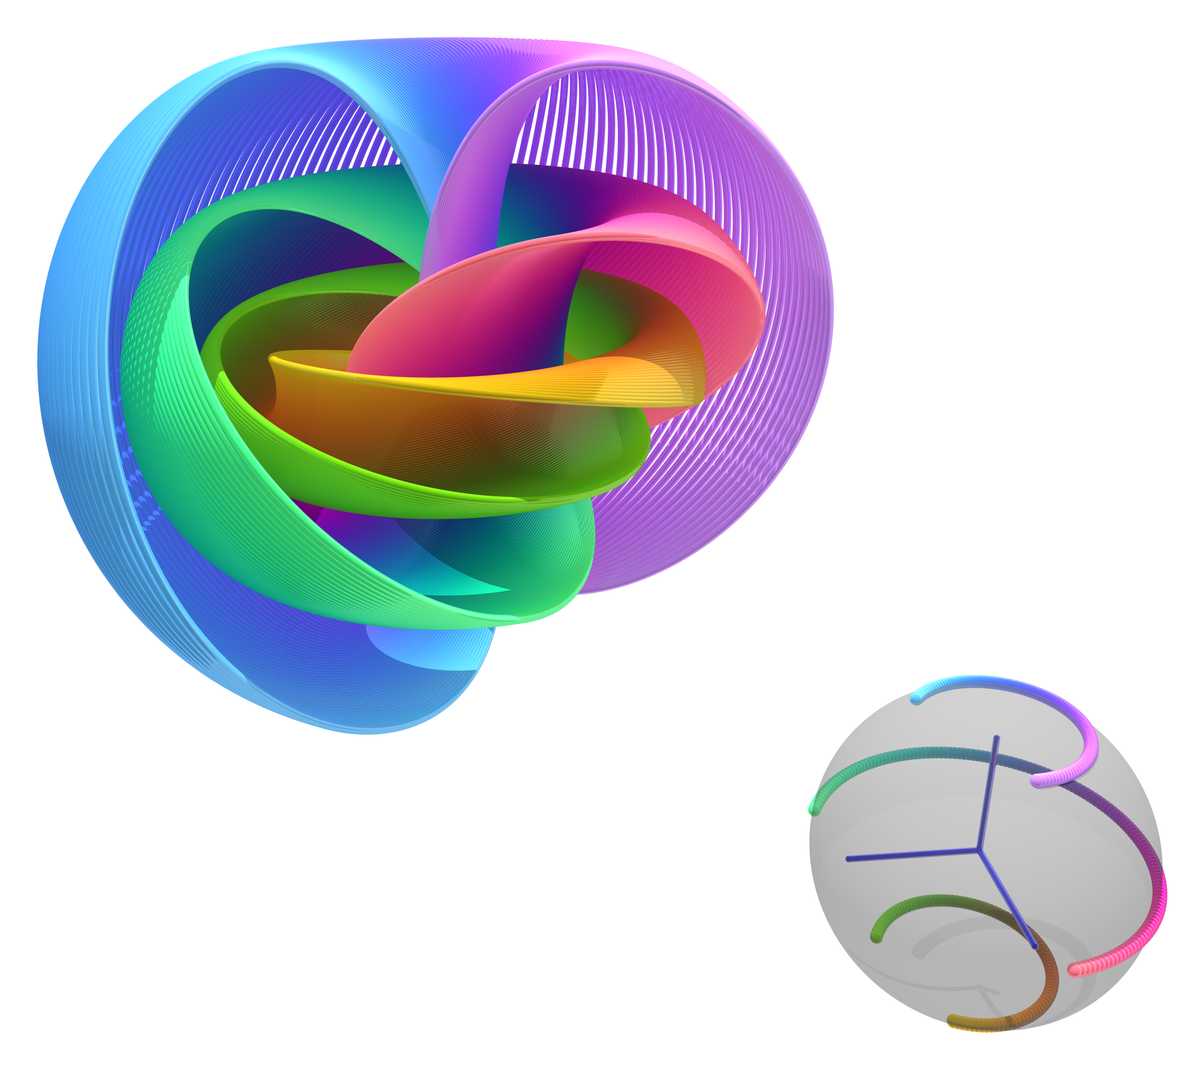
\includegraphics[width=0.70\textwidth]{figures/N-20251217/Hopf_Fibration.png}
  \caption{the Hopf fibration visualized by linked fibres.}
\end{figure}

The Hopf fibration matters because it is not null-homotopic.  It represents a nontrivial element of
\[
  \pi_3(S^2).
\]
In beginner language: even though \(S^3\) and \(S^2\) are both spheres, the map \(H:S^3\to S^2\) cannot be continuously shrunk to a constant map.

\begin{definition}[Null-homotopic map]
A map \(f:X\to Y\) is null-homotopic if it is homotopic to a constant map.  Equivalently, there is a continuous family of maps \(f_t:X\to Y\) with \(f_0=f\) and \(f_1\) constant.
\end{definition}

The Hopf map is the first warning: a process can be topologically nontrivial even if it looks, from far away, like a map between simple spaces.

\section{Homotopy groups and the first stable class}

For a based space \(X\), the group \(\pi_n(X)\) is made from based maps \(S^n\to X\), modulo based homotopy.  The lecture reviews the low-dimensional intuition:
\[
  \pi_0(X)=\text{connected components},
  \qquad
  \pi_1(X)=\text{loops modulo homotopy}.
\]
Higher homotopy groups generalize this to maps from higher-dimensional spheres.

For spheres, the groups are easy below the diagonal:
\[
  \pi_i(S^n)=0
  \qquad (i<n).
\]
On the diagonal, one has the degree:
\[
  \pi_n(S^n)\cong\mathbb Z.
\]
But above the diagonal the world becomes subtle.  The Hopf map gives the famous example
\[
  \pi_3(S^2)\neq0.
\]

The stable homotopy groups of spheres are obtained by repeatedly suspending:
\[
  \pi_i^s(\mathbb S)
  =
  \lim_{n\to\infty}\pi_{i+n}(S^n).
\]
The Hopf map contributes the first stable nontrivial class
\[
  \eta\in \pi_1^s(\mathbb S)\cong\mathbb Z/2.
\]
This class has order two: doing it twice becomes trivial, but doing it once is not trivial.

\section{From natural numbers to finite sets}

The lecture then changes viewpoint.  Instead of defining the natural numbers as primitive symbols, define them as isomorphism classes of finite sets:
\[
  \mathbb N
  \cong
  \pi_0(\mathrm{FinSet}).
\]
Here a finite set of size \(n\) represents the number \(n\).  Disjoint union represents addition:
\[
  A+B := A\sqcup B.
\]

To get the integers, one takes a group completion.  Informally, one allows formal differences
\[
  A-B.
\]
Thus the number \(1-1\) is represented by a pair consisting of one positive point and one negative point.

\begin{remark}
The corresponding slide phrases this as a move from numbers to finite sets: the natural number \(n\) is represented by an \(n\)-element set, and addition is represented by disjoint union.  This is the first categorification step in the lecture: instead of remembering only the cardinality, one keeps the finite set itself and later also its symmetries.
\end{remark}


\begin{definition}[Grothendieck group]
Given a commutative monoid \(M\), its Grothendieck group \(K_0(M)\) is the universal abelian group receiving a monoid homomorphism from \(M\).  For finite sets under disjoint union this gives
\[
  K_0(\mathrm{FinSet})\cong\mathbb Z.
\]
\end{definition}

So far, this still only explains the value of \(1-1\).  It does not yet explain why the path
\[
  0\to 1-1\to -1+1\to 0
\]
can be interesting.  For that, we must remember not just the set of isomorphism classes, but the space of finite sets and isomorphisms.

\section{The space of finite sets}

The slide deck asks us to consider the moduli space
\[
  \mathcal F=\mathrm{FinSet}/\sim.
\]
This is not merely a set of cardinalities.  It remembers automorphisms of finite sets.  A finite set with \(n\) elements has automorphism group \(S_n\), the symmetric group.

\begin{remark}
The slide at this point depicts the moduli space of finite sets as a space whose \(n\)-point component remembers \(S_n\).  In notebook language, the important formula is
\[
  \mathcal F\simeq \bigsqcup_{n\ge0}BS_n.
\]
Thus the component remembers the number \(n\), while loops in that component remember permutations.
\end{remark}


One can think of \(\mathcal F\) as a disjoint union of classifying spaces:
\[
  \mathcal F\simeq \bigsqcup_{n\ge0}BS_n.
\]
This formula is the first place where the hidden loops appear.  A point in \(BS_n\) remembers a finite set of size \(n\), but loops at that point remember permutations of the set.

Thus the finite set with one positive and one negative point is not just a cardinality-zero object.  It can have a nontrivial path coming from swapping the two labelled positions before annihilation.

\section[The K-space of finite signed sets]{The \(K\)-space of finite signed sets}

To group-complete finite sets at the level of spaces, the slides introduce a space \(K(\mathcal F)\).  Its points are finite ordered configurations whose elements are marked by \(+\) or \(-\).  Adjacent opposite signs may cancel.

\begin{remark}
The slide introduces the \(K\)-space by replacing finite sets with signed finite configurations.  The picture is simple enough to state in words: points marked \(+\) and points marked \(-\) may be created and cancelled in opposite-signed pairs, and the empty configuration is used as the base point.
\end{remark}


The empty configuration \(\varnothing\) is the base point.  The configuration \(\{+,-\}\) has total signed cardinality zero, but it is not identical to the empty configuration before one performs cancellation.  This distinction is the seed of the whole example.

The higher \(K\)-groups are defined by
\[
  K_i(\mathrm{FinSet})
  =
  \pi_i(K(\mathcal F),\varnothing).
\]
Thus \(K_0\) records components, while \(K_1\) records loops based at the empty configuration.

\section[The loop h]{The loop \(h\)}

Now the lecture constructs the loop
\[
  h:\varnothing
  \sim \{+,-\}
  \sim \{-,+\}
  \sim \varnothing.
\]
It has three stages.

First, create a cancelling pair:
\[
  \varnothing\longrightarrow \{+,-\}.
\]
Second, swap the two points:
\[
  \{+,-\}\longrightarrow \{-,+\}.
\]
Third, annihilate the cancelling pair:
\[
  \{-,+\}\longrightarrow \varnothing.
\]

\Needspace{14\baselineskip}
\begin{figure}[htbp]
  \centering
  \includegraphics[page=42,width=0.92\textwidth]{figures/N-20251217/zero-eq-zero-slides.pdf}
  \caption{From the lecture slides: the loop \(h\) represented by creation, swap, and annihilation.}
\end{figure}

This is the corrected meaning of
\[
  0=1-1=-1+1=0.
\]
It is not the claim that zero equals zero.  It is the claim that there is a particular loop at zero.  The middle step, the swap, is the nontrivial part.

\begin{remark}
If the two points were not moved, the movie would look like a boring creation followed by immediate annihilation.  The swap forces a braid-like motion.  In configuration space, this motion wraps around the collision locus where the two points would meet.
\end{remark}

The slides record the key computation:
\[
  K_1(\mathrm{FinSet})\cong\mathbb Z/2,
\]
and the loop \(h\) gives the nontrivial element.  Doing the swap twice is null-homotopic, but doing it once is not.

\section{Why this is not analytic summation}

At this point the earlier misreading can be corrected precisely.  Ces\`aro or Abel summation asks for a value of an infinite expression such as
\[
  1-1+1-1+\cdots.
\]
The lecture's loop is finite.  It uses one positive point and one negative point.  Its nontriviality is not caused by infinitely many cancellations.

The Eilenberg swindle is also different.  The swindle uses an infinite object that absorbs a copy of itself.  Here the point is not that a structure disappears at infinity.  The point is that a finite movie becomes nontrivial after stabilization.

So the corrected contrast is:
\[
\begin{array}{c|c}
\text{wrong centre of gravity} & \text{correct centre of gravity}\\
\hline
\text{value of a divergent sum} & \text{homotopy class of a loop}\\
\text{infinite cancellation} & \text{finite creation--swap--annihilation}\\
\text{forcing a number} & \text{detecting a stable topological class}
\end{array}
\]

\section{Finite sets and stable spheres}

The surprising theorem behind the example is the Barratt--Priddy--Quillen theorem.  In the form used by the lecture, it says that the \(K\)-theory of finite sets is the sphere spectrum:
\[
  K_i(\mathrm{FinSet})
  \cong
  \pi_i^s(\mathbb S).
\]

\begin{theorem}[Barratt--Priddy--Quillen, lecture form]
The \(K\)-theory of finite sets is the sphere spectrum.  Equivalently,
\[
  K_i(\mathrm{FinSet})\cong \pi_i^s(\mathbb S).
\]
\end{theorem}

In the slide deck this theorem is presented as the conceptual bridge: a finite-set loop can detect a stable homotopy class of spheres.


This theorem explains why the finite-set loop \(h\) can be compared to the Hopf class.  Under BPQ, the nontrivial element of
\[
  K_1(\mathrm{FinSet})\cong\mathbb Z/2
\]
corresponds to
\[
  \eta\in \pi_1^s(\mathbb S)\cong\mathbb Z/2.
\]
This is the stable Hopf class.

Another way to say this is that \(K(\mathcal F)\) can be seen as a stable configuration space of framed points:
\[
  K(\mathcal F)\simeq \mathrm{Conf}^{\mathrm{fr}}(\mathbb R^\infty).
\]
The creation--swap--annihilation loop becomes a framed one-dimensional motion.  Its framing carries the \(\mathbb Z/2\)-twist.

\section{Relation with the classical Hopf map}

The classical Hopf fibration represents a nontrivial element of \(\pi_3(S^2)\).  Stabilizing the Hopf map gives the stable element
\[
  \eta\in \pi_1^s(\mathbb S).
\]
The finite-set loop \(h\) gives the same class under the BPQ theorem.

Thus the meme ladder is not merely free association.  The chain is:
\[
\begin{array}{c}
\text{Hopf fibration }S^3\to S^2\\
\Downarrow\\
\text{stable Hopf element }\eta\in\pi_1^s(\mathbb S)\\
\Downarrow\\
K_1(\mathrm{FinSet})\cong\pi_1^s(\mathbb S)\\
\Downarrow\\
\text{the loop }h:\varnothing\sim\{+,-\}\sim\{-,+\}\sim\varnothing.
\end{array}
\]

This is the clean mathematical sense in which the arithmetic-looking line is the Hopf map in disguise.

\section{Cobordism: the movie becomes a circle}

The slides then place the motion in three-dimensional space.  As time evolves, the moving point configuration sweeps out a one-dimensional manifold.  The creation of the pair, their swap, and their annihilation form a closed loop.  Because the points carry signs or framings, the resulting circle is a framed one-manifold.

\Needspace{14\baselineskip}
\begin{figure}[htbp]
  \centering
  \includegraphics[page=53,width=0.92\textwidth]{figures/N-20251217/zero-eq-zero-slides.pdf}
  \caption{From the lecture slides: the creation--swap--annihilation movie becomes a framed circle.}
\end{figure}

Framed cobordism asks whether this framed circle is the boundary of a framed disk.  The answer is no for the loop \(h\).  This is another expression of the same nontrivial \(\mathbb Z/2\)-class.

\begin{definition}[Framed cobordism, informal]
A framed \(n\)-manifold is an \(n\)-manifold equipped with a trivialization of its normal bundle.  Two framed manifolds are framed cobordant if they form the boundary of a framed manifold one dimension higher.
\end{definition}

This is the geometric face of the equation.  The path starts and ends at the empty configuration, but its trace is not the boundary of a trivial framed disk.  The loop is geometrically nonzero.

\section[Algebraic K-theory of a field]{Algebraic \(K\)-theory of a field}

After finite sets, the lecture repeats the construction with finite-dimensional vector spaces over a field \(k\).  Let
\[
  \mathcal V_k=\mathrm{FinVect}_k/\sim
\]
be the moduli space of finite-dimensional vector spaces.  Under direct sum, it behaves like a categorified version of addition.

The low \(K\)-groups are familiar:
\[
  K_0(k)\cong\mathbb Z,
  \qquad
  K_1(k)\cong k^\times.
\]
The first says that a vector space is measured by its dimension after group completion.  The second says that the determinant detects the abelianized automorphism information:
\[
  \mathrm{GL}_\infty(k)^{\mathrm{ab}}\cong k^\times.
\]

This parallels the finite-set case:
\[
\begin{array}{c|c|c}
\text{object} & K_0 & K_1\\
\hline
\mathrm{FinSet} & \mathbb Z & \mathbb Z/2\\
\mathrm{FinVect}_k & \mathbb Z & k^\times
\end{array}
\]
The lecture now asks for a geometric model of these algebraic \(K\)-groups beyond degree one.

\section{Intrinsic skein-lasagna}

The advanced second half of the slide deck introduces intrinsic skein-lasagna.  This is not merely decorative.  It is a proposed geometric language for \(K\)-groups analogous to how framed cobordism gives a geometric language for stable homotopy.

The first definition is an \(n\)-treefold: a space locally homeomorphic to
\[
  T\times \mathbb R^{n-1},
\]
where \(T\) is a tree.  The branching models a controlled kind of singularity.

Given a symmetric monoidal category \((\mathcal C,\otimes)\), an \(n\)-\((\mathcal C,\otimes)\)-lasagna is, roughly, a framed \(n\)-treefold with labels from \(\mathcal C\), satisfying compatibility at the branching loci.

\begin{definition}[Intrinsic skein-lasagna, informal]
An intrinsic lasagna is a geometric object built from treefold-like pieces, with labels coming from a symmetric monoidal category.  The word ``intrinsic'' means that the object is studied on its own, rather than as something embedded in a previously chosen ambient manifold.
\end{definition}

The slide illustrates \(n\)-treefolds as spaces locally modelled on \(T\times\mathbb R^{n-1}\), where \(T\) is a tree.  For the notebook, the useful point is that branching is allowed but controlled.


The word ``intrinsic'' is important.  Classical skein-lasagna modules often involve embedded objects inside an ambient manifold.  Here the lecture emphasizes that one can study the geometry of the lasagna itself, without first choosing an ambient space.  If desired, one may imagine the ambient space as \(\mathbb R^\infty\), but it is no longer part of the primary data.

\section[The V-k cobordism group]{The \((\mathcal V_k,\oplus)\)-cobordism group}

The lecture specializes the lasagna story to
\[
  (\mathcal V_k,\oplus),
\]
where \(\mathcal V_k\) is the category or moduli object of finite-dimensional vector spaces under direct sum.  One obtains groups denoted
\[
  \Omega_n^{\mathcal V_k,\oplus}.
\]
The examples in low degree match algebraic \(K\)-theory:
\[
  \Omega_0^{\mathcal V_k,\oplus}\cong K_0(k)\cong\mathbb Z,
\]
\[
  \Omega_1^{\mathcal V_k,\oplus}\cong K_1(k)\cong k^\times.
\]

\begin{remark}
The slide summarizes the first two \((\mathcal V_k,\oplus)\)-cobordism groups: degree \(0\) recovers dimension, and degree \(1\) recovers determinant.  In formulas,
\[
  \Omega_0^{\mathcal V_k,\oplus}\cong K_0(k)\cong\mathbb Z,
  \qquad
  \Omega_1^{\mathcal V_k,\oplus}\cong K_1(k)\cong k^\times.
\]
This is why vector-space-labelled circles are the \(K_1\) analogue of the finite-set swap loop.
\end{remark}


The degree-one case is especially helpful.  A circle labelled by an automorphism \(f\in\mathrm{GL}(V)\) represents a class, and the determinant gives its value in \(k^\times\).  A commutator becomes null-cobordant, matching the abelianization of \(\mathrm{GL}_\infty(k)\).

This is the lasagna analogue of the finite-set story.  In finite sets, a swap gives the nontrivial element of \(\mathbb Z/2\).  In vector spaces, an automorphism gives an element of \(k^\times\).

\section{Generalized Pontryagin--Thom}

The slide deck then states the central claim:
\[
  K_n(k)\xrightarrow{\cong}\Omega_n^{\mathcal V_k,\oplus}
  \qquad (n\ge0).
\]
This is presented as a generalized Pontryagin--Thom isomorphism.

\Needspace{14\baselineskip}
\begin{figure}[htbp]
  \centering
  \includegraphics[page=69,width=0.92\textwidth]{figures/N-20251217/zero-eq-zero-slides.pdf}
  \caption{From the lecture slides: the generalized Pontryagin--Thom isomorphism identifies \(K_n(k)\) with a lasagna-cobordism group.}
\end{figure}

The analogy is:
\[
\begin{array}{c|c}
\text{classical/stable homotopy} & \text{algebraic \(K\)-theory side}\\
\hline
\pi_n^s(\mathbb S) & K_n(k)\\
\Omega_n^{\mathrm{fr}} & \Omega_n^{\mathcal V_k,\oplus}\\
\text{framed manifolds} & \text{vector-space-labelled lasagnas}
\end{array}
\]
This is why the lecture moves from elementary arithmetic to Hopf fibration and then to intrinsic skein-lasagna.  It is building a geometric model of algebraic \(K\)-theory.

\section[The K2 slide and Steinberg relations]{The \(K_2\) slide and Steinberg relations}

In degree two, the lecture recalls the classical presentation
\[
  K_2(k)
  \cong
  k^\times\otimes k^\times/
  \langle a\otimes(1-a)\rangle.
\]
It then considers matrices \(f,g\in\mathrm{GL}(k)\) with commutator
\[
  [f,g]=1.
\]
Such a commuting pair defines a two-dimensional lasagna \(C(f,g)\).

\Needspace{14\baselineskip}
\begin{figure}[htbp]
  \centering
  \includegraphics[page=72,width=0.92\textwidth]{figures/N-20251217/zero-eq-zero-slides.pdf}
  \caption{From the lecture slides: a two-lasagna \(C(f,g)\) associated to a commuting pair.}
\end{figure}

The next slide gives a more concrete example using elementary matrices.  For \(i\ne j\), let
\[
  e_{ij}(a)
\]
be the elementary matrix with \(a\) in the \((i,j)\)-entry and ones on the diagonal.  These matrices satisfy Steinberg relations, such as
\[
  [e_{ij}(a),e_{kl}(b)]
  =
  \begin{cases}
  e_{il}(ab), & j=k,\\
  \mathbf 1, & \text{otherwise.}
  \end{cases}
\]
The slide then uses Hall--Witt-type commutator identities to produce a nontrivial proof that a certain commutator is the identity.  This proof is not just algebraic decoration; it is a blueprint for constructing a bounding three-lasagna.

\Needspace{14\baselineskip}
\begin{figure}[htbp]
  \centering
  \includegraphics[page=75,width=0.92\textwidth]{figures/N-20251217/zero-eq-zero-slides.pdf}
  \caption{From the lecture slides: elementary matrices, Steinberg relations, and the algebraic pattern behind the three-lasagna.}
\end{figure}

\section{The final lasagna diagrams}

The final nontrivial slides display a Heegaard splitting and a boundary relation.  They are not necessary for understanding the original meme, but they are essential for understanding where the lecture is going.  The creation--swap--annihilation loop was the baby example.  The lasagna diagrams are the research-level continuation of the same philosophy: algebraic \(K\)-theory classes are represented by geometric/cobordism-like objects.

\Needspace{14\baselineskip}
\begin{figure}[htbp]
  \centering
  \includegraphics[page=78,width=0.92\textwidth]{figures/N-20251217/zero-eq-zero-slides.pdf}
  \caption{From the lecture slides: a Heegaard-splitting picture used to construct a three-lasagna.}
\end{figure}

\Needspace{14\baselineskip}
\begin{figure}[htbp]
  \centering
  \includegraphics[page=79,width=0.92\textwidth]{figures/N-20251217/zero-eq-zero-slides.pdf}
  \caption{From the lecture slides: the boundary relation for the three-lasagna construction.}
\end{figure}

At this point the lecture has travelled very far from the original equation.  But the path is coherent:
\[
\begin{array}{c}
\text{equation as path}\\
\Downarrow\\
\text{finite signed configurations}\\
\Downarrow\\
\text{\(K\)-theory of finite sets}\\
\Downarrow\\
\text{stable homotopy and framed cobordism}\\
\Downarrow\\
\text{algebraic \(K\)-theory of fields}\\
\Downarrow\\
\text{intrinsic skein-lasagna as a geometric model.}
\end{array}
\]

\section{What the equation finally says}

The equation
\[
  0=1-1=-1+1=0
\]
should be read as the name of a loop:
\[
  h:\varnothing\to\{+,-\}\to\{-,+\}\to\varnothing.
\]
It is a loop at zero in the \(K\)-space of finite sets.  It is not the identity loop.  It represents the generator of
\[
  K_1(\mathrm{FinSet})\cong\mathbb Z/2.
\]
By Barratt--Priddy--Quillen, this group is
\[
  \pi_1^s(\mathbb S)\cong\mathbb Z/2,
\]
and \(h\) corresponds to the stable Hopf class \(\eta\).

This is why the Hopf fibration belongs in the same story as a signed finite-set calculation.  The shared object is not an ordinary number.  It is a stable homotopy class.

\section{Structural viewpoint}

The first note preserved the background: a summer memory, a lecture poster, and a mistaken attempt to decode a meme.  This second note gives the corrected mathematical reading.

The hierarchy is:
\[
\begin{array}{c|c}
\text{naive reading} & \text{corrected reading}\\
\hline
0=0 & \text{a loop from \(0\) to \(0\)}\\
1-1 & \text{a created \(+\)/\(-\) pair}\\
-1+1 & \text{the same pair after a swap}\\
\text{arithmetic cancellation} & \text{creation--swap--annihilation movie}\\
\text{divergent summation} & \text{\(K_1(\mathrm{FinSet})\)}\\
\text{meme punchline} & \text{stable Hopf class \(\eta\)}
\end{array}
\]

The advanced tail of the lecture should also be remembered.  The same style of thought continues beyond finite sets.  For a field \(k\), algebraic \(K\)-groups can be approached through vector-space-labelled lasagnas:
\[
  K_n(k)\cong \Omega_n^{\mathcal V_k,\oplus}.
\]
The final slides are not random extra material.  They show that the playful equation is the doorway into a geometric model of algebraic \(K\)-theory.

So the final lesson is not that \(0\) is secretly nonzero.  The lesson is that in higher mathematics, the space of ways for \(0\) to be \(0\) can contain a nontrivial loop.
